% Official IEEE Signal Processing Magazine Columns & Forum submission format.
% Template package: IEEE-SPM-C&F-Templates_LaTeX.zip, retrieved from the
% IEEE Template Selector on September 2, 2026.
\documentclass[11pt,draftcls,onecolumn,journal]{IEEEtran}

\usepackage{amsmath,amsfonts}
\usepackage{algorithmic}
\usepackage{algorithm}
\usepackage{float}
\usepackage{array}
\usepackage[caption=false,font=normalsize,labelfont=sf,textfont=sf]{subfig}
\usepackage{textcomp}
\usepackage{stfloats}
\usepackage{url}
\usepackage{verbatim}
\usepackage{graphicx}
\usepackage{cite}
\usepackage{xcolor}
\usepackage{bm}
\usepackage[hidelinks]{hyperref}
\usepackage{booktabs}
\hyphenation{op-tical net-works semi-conduc-tor IEEE-Xplore}
\hypersetup{
  pdftitle={A First-Order Cyclostationarity Statistic Is a Tone Matched-Filter GLRT},
  pdfauthor={Dylan J. Gormley},
  pdfsubject={First-order cyclostationarity, cyclic means, Fourier coefficients, and tone matched filtering}
}

\definecolor{deepblue}{HTML}{194C80}
\definecolor{warmgray}{HTML}{F2F3F5}

\newcommand{\E}{\mathbb{E}}
\newcommand{\CN}{\mathcal{CN}}
\newcommand{\vect}[1]{\bm{#1}}

\title{A First-Order Cyclostationarity Statistic Is a Tone Matched-Filter GLRT\\
{\large The Equivalence Chain and Its Conditions}}

\author{Dylan~J.~Gormley and Kevin~M.~Bandura%
\thanks{This work was supported by the National Science Foundation under grant number 2307581.
Dylan J. Gormley and Kevin~M.~Bandura are with West Virginia University's Department of Computer Science \& Electrical Engineering in Morgantown, WV, USA.  %
\{\href{mailto:dylan.gormley@mail.wvu.edu}{dylan.gormley}, \href{mailto:kevin.bandura@mail.wvu.edu}{kevin.bandura}\}@mail.wvu.edu
}%
}

\markboth{IEEE Signal Processing Magazine, Columns \& Forum Draft}%
{Gormley: A First-Order Cyclostationarity Statistic}

\begin{document}
\maketitle
\section*{}
\label{sec:introduction}
\IEEEPARstart{C}{yclostationarity} is usually introduced through second- and higher-order statistics, so its first-order member is easy to overlook.  Yet first order gives an unusually simple connection.  Its cyclic moment is the cyclic mean, and a finite-record cyclic-mean estimate counter-rotates the data and averages.  That operation is also a discrete-time Fourier transform (DTFT) evaluation and a complex-tone correlation; on the discrete Fourier transform (DFT) grid, it is a DFT coefficient.  Under a known-frequency tone model in proper complex white Gaussian noise of known variance, the noise-normalized squared magnitude of this same output is a generalized likelihood-ratio test (GLRT) statistic for an unknown complex amplitude.

The result is not a new detector.  Its value is the translation: a first-order cyclic feature can be implemented, analyzed, and checked using familiar tone-detection machinery.  The same translation also identifies the limits of the claim---FFT gridding belongs to the implementation, optimality belongs to the noise and signal model, and interpretation as an ensemble cyclic mean requires phase coherence or an appropriate consistency condition.  This article derives the identity, verifies its finite-sample detection law, and turns those distinctions into a short practical guide.

\section*{The Core Operation: Counter-Rotate, Then Average}

At first order, the cyclic moment is the cyclic mean.  Its finite-record estimate is obtained by counter-rotating at the candidate cycle frequency and averaging---the same operation that evaluates a finite-record DTFT sample and correlates the record with a complex tone.  Consider the complex record $x[0],\ldots,x[N-1]$, and let $\alpha\in[-1/2,1/2)$ denote the candidate frequency in cycles per sample.  An ordinary sample mean extracts zero frequency, so a component at nonzero $\alpha$ is generally attenuated by phase cancellation.  Define the phase-corrected samples as $z_{\alpha}[n]\equiv x[n]e^{-j2\pi\alpha n}$.  A matching component then moves to zero frequency, and the finite-record cyclic-mean estimate is the ordinary sample mean of the corrected sequence:
\begin{equation}
\widehat R_{x,1}^{\alpha}(0)
\equiv\widehat M_x^{\alpha}
=\frac{1}{N}\sum_{n=0}^{N-1}z_{\alpha}[n]
=\frac{1}{N}\sum_{n=0}^{N-1}x[n]e^{-j2\pi\alpha n}.
\label{eq:cyclicmean}
\end{equation}
Here, $M_x^{\alpha}$ denotes the underlying time-average or ensemble coefficient, $\widehat M_x^{\alpha}$ denotes its finite-record estimate, and the decision statistic $T_{\alpha}$ will be defined below.  For example, if $x[n]=ae^{j2\pi\alpha n}$, then $z_{\alpha}[n]=a$ for every $n$ and $\widehat M_x^{\alpha}=a$.  A frequency mismatch leaves a residual phase progression and attenuates the average through phase cancellation.  This first-order estimator is also used directly in cyclostationary signal detection and classification~\cite[eq. (9)]{dobre2009}.

\textbf{Fourier and correlator views.}
Writing the phase-correction weights as vectors makes the connection explicit.  Collect the record and candidate phase progression in
\begin{equation}
\begin{aligned}
\vect{x}
&=\begin{bmatrix}
x[0] & x[1] & \cdots & x[N-1]
\end{bmatrix}^{T},\\
\vect{s}_{\alpha}
&=\begin{bmatrix}
1 & e^{j2\pi\alpha} & \cdots & e^{j2\pi\alpha(N-1)}
\end{bmatrix}^{T}.
\end{aligned}
\end{equation}
The entries of $\vect{s}_{\alpha}^{H}$ are exactly the phase-correction factors in~\eqref{eq:cyclicmean}, so
\begin{equation}
N\widehat M_x^{\alpha}=\vect{s}_{\alpha}^{H}\vect{x}.
\label{eq:identity}
\end{equation}

Let $X_N(\alpha)\equiv\sum_{n=0}^{N-1}x[n]e^{-j2\pi\alpha n}$ denote the length-$N$ DTFT evaluation.  Equation~\eqref{eq:identity} exposes the finite-record chain:
\begin{equation}
\widehat M_x^{\alpha}
=\frac{X_N(\alpha)}{N}
=\frac{\vect{s}_{\alpha}^{H}\vect{x}}{N}.
\label{eq:chain}
\end{equation}
For an integer DFT index $k$, let $\alpha_k$ be the representative of $k/N$ in $[-1/2,1/2)$.  Periodicity then gives $X_N(\alpha_k)=N\widehat M_x^{\alpha_k}=X[k]$, where
\begin{equation}
X[k]=\sum_{n=0}^{N-1}x[n]e^{-j2\pi kn/N}.
\end{equation}
For arbitrary $\alpha$, the sum remains an exact DTFT evaluation, but it is not generally an $N$-point DFT coefficient.  Zero padding evaluates the same DTFT exactly on a denser FFT grid; interpolation or frequency refinement approximates an arbitrary off-grid location.  This is the ordinary FFT-grid issue, not a restriction of the first-order identity.  Gardner's time-average Fourier coefficients provide the corresponding infinite-record view~\cite[eqs. (1)--(3)]{gardner1986}.

\begin{center}
\fcolorbox{deepblue}{warmgray}{%
\begin{minipage}{0.88\textwidth}
\textbf{The tip.} When the feature of interest is first order, no specialized cyclostationary processing block is needed: compute the familiar tone correlation in~\eqref{eq:chain}.  Under the white-Gaussian model below, its noise-normalized squared magnitude also inherits the standard tone-GLRT threshold and performance expressions.
\end{minipage}}
\end{center}

\section*{Why the First-Order Member Is the Cyclic Mean}

Using the continuous-time convention of the source, the name follows from the general $p$th-order cyclic temporal cross-moment~\cite[eq. (13.1)]{gardner2006}:
\begin{equation}
R_{x,p}^{\alpha}(\vect{\tau})
=
\left\langle
\prod_{\ell=1}^{p}
x_{\ell}^{(*)_{\ell}}(t+\tau_{\ell})
e^{-j2\pi\alpha t}
\right\rangle_t ,
\label{eq:general}
\end{equation}
Here, $p$ is the moment order, $(*)_{\ell}$ denotes optional conjugation, $\vect{\tau}$ contains the $p$ delays of the full representation, and $\langle\cdot\rangle_t$ denotes a time average.  When $p=1$, the product contains one factor, so the first-order cyclic moment is the cyclic mean.  It is the order-one member of the generalized cyclic-moment hierarchy, but no separate spectral-frequency coordinate remains: the reduced-dimension representation of a $p$th-order moment has $p-1$ independent relative lags, and at $p=1$ there is no independent relative-lag variable to Fourier transform.  Optional conjugation does not create an independent statistic over a two-sided cycle-frequency domain because
\begin{equation*}
\left\langle x^*(t+\tau)e^{-j2\pi\alpha t}\right\rangle_t
=
\left[
\left\langle x(t+\tau)e^{+j2\pi\alpha t}\right\rangle_t
\right]^* .
\end{equation*}
Thus, the unconjugated coefficients at both signs of $\alpha$ determine the conjugated coefficients; for real-valued $x$, the forms coincide at each cycle frequency.  The reduced-dimension form fixes one reference delay at zero~\cite[eq. (13.7)]{gardner2006}.  At first order, $\tau$ is therefore a common time shift rather than a relative-lag coordinate.  Shift invariance of the infinite-time average gives
\begin{equation*}
R_{x,1}^{\alpha}(\tau)
=\left\langle x(t+\tau)e^{-j2\pi\alpha t}\right\rangle_t
=R_{x,1}^{\alpha}(0)e^{j2\pi\alpha\tau}.
\end{equation*}
This common shift changes the coefficient only by the known phase $e^{j2\pi\alpha\tau}$.  Adopting the reduced-dimension convention $\tau=0$ therefore loses no information, and the time-average first-order cyclic moment, or cyclic mean, is
\begin{equation}
M_x^{\alpha}
\equiv R_{x,1}^{\alpha}(0)
=\left\langle x(t)e^{-j2\pi\alpha t}\right\rangle_t .
\label{eq:cyclicmeanct}
\end{equation}

Equation~\eqref{eq:cyclicmean} is its sampled, rectangular, $N$-sample finite-record estimate.  Treating it as a consistent estimate of an ensemble cyclic mean additionally requires a specified phase convention and an appropriate first-order cycloergodicity or consistency condition, as discussed below.

\section*{When the Common Output Is a GLRT}

The identities above are algebraic; they do not by themselves establish detector optimality.  We now state the signal and noise model under which the common correlation yields the GLRT~\cite[Sec. 13.4.1]{kay1998}.  The same tone-detection connection is also developed from matched-filter and Fourier viewpoints in~\cite[p. 600]{spooner2009}:
\begin{align}
\mathcal H_0 &: \vect{x}=\vect{w},\nonumber\\
\mathcal H_1 &: \vect{x}=a\vect{s}_{\alpha}+\vect{w},
\qquad
\vect{w}\sim\CN(\vect{0},\sigma^2\vect{I}),
\label{eq:model}
\end{align}
Here, the normalized frequency $\alpha$ and noise variance $\sigma^2$ are known, the deterministic complex amplitude $a$ is unknown, and the noise is proper (circularly symmetric) complex white Gaussian.  Our variance convention is $\E\{\vect{w}\vect{w}^{H}\}=\sigma^2\vect{I}$ and $\E\{\vect{w}\vect{w}^{T}\}=\vect{0}$.  Apart from constants, the log likelihood is
\begin{equation}
\ell(a)=-\frac{1}{\sigma^2}
\left\|\vect{x}-a\vect{s}_{\alpha}\right\|^2 .
\end{equation}
We complete the square and use $\vect{s}_{\alpha}^{H}\vect{s}_{\alpha}=N$ to obtain the maximum-likelihood estimate
\begin{equation}
\widehat a
=\frac{\vect{s}_{\alpha}^{H}\vect{x}}
{\vect{s}_{\alpha}^{H}\vect{s}_{\alpha}}
=\widehat M_x^{\alpha},
\label{eq:ahat}
\end{equation}
Substituting~\eqref{eq:ahat} into the likelihood produces a GLRT that is monotone in
\begin{equation}
T_{\alpha}
=\frac{|\vect{s}_{\alpha}^{H}\vect{x}|^2}
{\sigma^2\vect{s}_{\alpha}^{H}\vect{s}_{\alpha}}
=\frac{N|\widehat M_x^{\alpha}|^2}{\sigma^2}.
\label{eq:glrt}
\end{equation}

Equation~\eqref{eq:glrt} is an exact finite-sample result.  Under~\eqref{eq:model}, $T_{\alpha}$ is simultaneously noise-normalized cyclic-mean energy, a normalized periodogram ordinate, and a standard noncoherent tone-GLRT statistic.  The two-real-component covariance test below is $2T_{\alpha}$, so the numerical normalizations differ but the rejection regions are identical after threshold scaling.

We obtain the same conclusion from the covariance-normalized form used for statistical cyclic-feature tests~\cite[eqs. (B.1)--(B.3)]{dobre2009}.  Let
\begin{equation}
\widehat{\vect{m}}
=\begin{bmatrix}
\Re\{\widehat M_x^{\alpha}\} &
\Im\{\widehat M_x^{\alpha}\}
\end{bmatrix}^{T}.
\end{equation}
Under $\mathcal H_0$,
$\operatorname{cov}(\widehat{\vect{m}})=\sigma^2\vect{I}_2/(2N)$, so
\begin{equation}
\widehat{\vect{m}}^{T}
\operatorname{cov}(\widehat{\vect{m}})^{-1}
\widehat{\vect{m}}
=\frac{2N|\widehat M_x^{\alpha}|^2}{\sigma^2}
=2T_{\alpha}.
\end{equation}
The positive factor of two changes only the threshold scale.  For one channel, Kay's complex-envelope sinusoid GLRT uses the same statistic with the corresponding factor-of-two threshold convention~\cite[eqs. (13.49)--(13.53)]{kay1998}.

We next determine the threshold from the null distribution.  Using the complex-noise convention in~\eqref{eq:model}, $T_{\alpha}$ has a unit-mean exponential distribution under $\mathcal H_0$.  Therefore,
\begin{equation}
P_{\mathrm{FA}}=e^{-\gamma},
\qquad
\gamma=-\log P_{\mathrm{FA}}.
\label{eq:pfa}
\end{equation}
\begin{samepage}
The direct implementation has three steps:
\begin{enumerate}
\item Counter-rotate and sum: $u_{\alpha}=\vect{s}_{\alpha}^{H}\vect{x}$.
\item Normalize: $T_{\alpha}=|u_{\alpha}|^2/(N\sigma^2)$.
\item Threshold: decide $\mathcal H_1$ when $T_{\alpha}>\gamma$.
\end{enumerate}
The final step is exact for one preassigned $\alpha$ when $\sigma^2$ is known.  If the variance is estimated, the null distribution and threshold must account for the variance estimator and any independent training data.
\end{samepage}
Under $\mathcal H_1$,
\begin{equation}
2T_{\alpha}\sim
\chi'^2_2\!\left(\frac{2N|a|^2}{\sigma^2}\right),
\label{eq:noncentral}
\end{equation}
which gives the standard noncoherent matched-filter detection probability.  Therefore, classical tone-detection performance expressions can be applied directly to the test based on $T_{\alpha}$.

If $a$, including its phase, is known, the Neyman-Pearson statistic is instead the coherent quantity
$\Re\{a^*\vect{s}_{\alpha}^{H}\vect{x}\}$.  The finite-record estimate $\widehat M_x^{\alpha}$ remains a scaled version of the sufficient complex matched-filter output.  However, the scalar decision statistic changes with the nuisance-parameter model.

\begin{table}[H]
\centering
\caption{What is exact, what is grid-specific, and what is statistical.}
\label{tab:names}
\renewcommand{\arraystretch}{1.25}
\begin{tabular}{>{\raggedright\arraybackslash}p{0.18\textwidth}
                >{\raggedright\arraybackslash}p{0.33\textwidth}
                >{\raggedright\arraybackslash}p{0.36\textwidth}}
\toprule
Role & Statement & What matters \\
\midrule
Core identity & $\widehat M_x^{\alpha}=X_N(\alpha)/N=\vect{s}_{\alpha}^{H}\vect{x}/N$ & Exact at every candidate $\alpha$; no FFT grid is required. \\
Shared FFT-grid issue & $\widehat M_x^{\alpha_k}=X[k]/N$ & A single $N$-point bin gives the exact sample when $\alpha\equiv k/N\pmod 1$.  Off grid, evaluate the DTFT directly or use the same denser-grid interpolation or refinement used in conventional cyclic-spectrum processing; this is not unique to first order. \\
Detector consequence & $T_{\alpha}=N|\widehat M_x^{\alpha}|^2/\sigma^2$ & The stated GLRT assumes one preassigned $\alpha$ and the white-noise tone model.  A frequency search changes the false-alarm threshold; colored noise uses the standard whitened form. \\
\bottomrule
\end{tabular}
\end{table}

The first row is the algebraic bridge, and the third row is the detector consequence stated in the title.  Only the DFT-bin shortcut in the middle row requires $\alpha\equiv k/N\pmod 1$; the cyclic-mean, DTFT, and tone-correlator identity remains exact off grid.  Thus, the grid condition qualifies an FFT implementation, while the final row's assumptions qualify optimality and thresholding.

\section*{Numerical Verification and Grid Mismatch}

We first verify the common statistic using a length-$64$ complex tone in white noise.  The simulation computes $T_{\alpha}$ independently from its counter-rotate-and-average and matched-filter forms, with a maximum absolute difference below $5\times10^{-12}$.  Following this direct check, we perform $80{,}000$ Monte Carlo trials per SNR value at $P_{\mathrm{FA}}=0.01$ using random seed 20260902 and per-sample SNR $\rho=|a|^2/\sigma^2$.  As shown in Figure~\ref{fig:verification}(a), the detection probability follows the noncentral chi-square law derived above.  The script and version-pinned direct-dependency list used to reproduce Figure~\ref{fig:verification} are available at \url{https://github.com/djgormley/fos}.

Next, we evaluate $T_{\alpha}$ at a single DFT bin.  This bin is matched only to its center frequency.  For the rectangular $N=64$ record used here, a half-bin tone offset has the exact power factor $[N\sin(\pi/(2N))]^{-2}$, or $-3.92$ dB, as shown in Figure~\ref{fig:verification}(b).  In comparison, direct evaluation of the cyclic mean at the true $\alpha$ remains exactly tuned.  A zero-padded FFT reduces the grid spacing; interpolation or frequency refinement can then estimate the off-grid peak.  These are the same choices made in FFT-based higher-order cyclic-spectrum processing.

\begin{figure}[H]
\centering
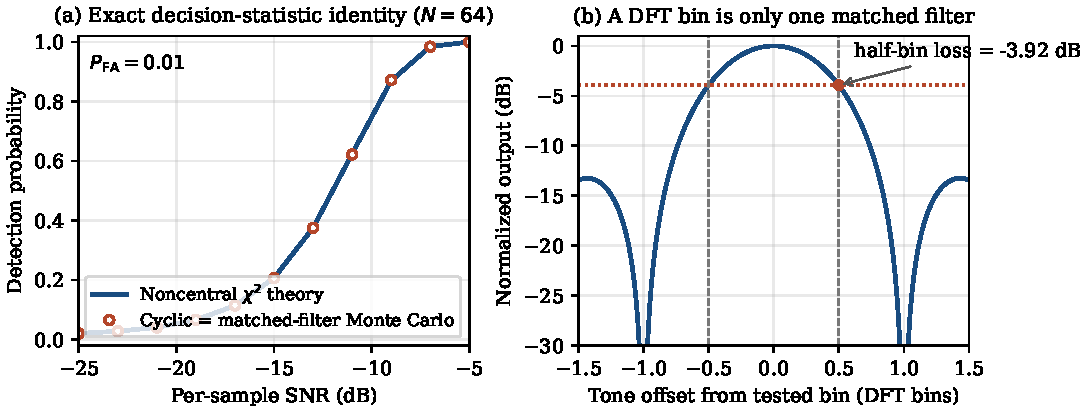
\includegraphics[width=0.98\textwidth]{equivalence_simulation.pdf}
\caption{(a) Monte Carlo detection probability for the common statistic $T_{\alpha}$.  The theoretical curve uses the threshold in~\eqref{eq:pfa} and the distribution in~\eqref{eq:noncentral}.  (b) Evaluating the statistic at only one DFT bin introduces rectangular-window mismatch loss.  The repository script reproduces both results.}
\label{fig:verification}
\end{figure}

\section*{Where the Equivalence Needs Care}

The finite-record identity holds independently of a stochastic model.  The following standard extensions modify the detector implementation, while the final caveat concerns interpretation as an ensemble cyclic mean.

\textbf{Unknown frequency.}
If the frequency is unknown, we maximize~\eqref{eq:glrt} over a candidate set:
\begin{equation}
T=\sup_{\alpha\in\mathcal A}
\frac{|\vect{s}_{\alpha}^{H}\vect{x}|^2}{N\sigma^2}.
\end{equation}
This operation is a bank of tone matched filters, also known as a peak-periodogram detector.  It is an FFT-bin search only when $\mathcal A$ is the DFT grid.  The false-alarm threshold must also account for the search; Equation~\eqref{eq:pfa} assumes that one preassigned trial frequency is tested.

\textbf{Colored noise.}
For colored noise with known positive-definite covariance $\vect{C}$ and $\vect{w}\sim\CN(\vect{0},\vect{C})$, the GLRT becomes
\begin{equation}
T_C=
\frac{|\vect{s}_{\alpha}^{H}\vect{C}^{-1}\vect{x}|^2}
{\vect{s}_{\alpha}^{H}\vect{C}^{-1}\vect{s}_{\alpha}}.
\label{eq:colored}
\end{equation}
Equation~\eqref{eq:colored} is the matched filter after whitening.  Therefore, the unwhitened cyclic-mean estimate or DFT coefficient is generally not optimal in colored noise.  The unwhitened statistic remains optimal when $\vect{s}_{\alpha}$ is an eigenvector of $\vect{C}$; this includes white noise and DFT-grid exponentials under a circulant covariance model.

\textbf{Real tones.}
For a real-valued record containing a known-frequency real sinusoid in real white Gaussian noise, the unknown-amplitude-and-phase GLRT projects onto the sine--cosine subspace.  At a non-DC, non-Nyquist DFT bin, these quadratures are orthogonal and the statistic is proportional to $|X[k]|^2$.  Off grid, we must retain the full Gram-matrix normalization rather than assume it is diagonal.

\textbf{Random ensemble phase.}
Lastly, we consider what is meant by ``first-order cyclostationarity.''  Let
\begin{equation}
X[n]=Ae^{j(2\pi\alpha_0 n+\Phi)}+W[n],
\qquad \Phi\sim\operatorname{Unif}[0,2\pi),
\label{eq:randomphase}
\end{equation}
where $A$ is deterministic, $W[n]$ is zero mean, and $\Phi$ is drawn once and held constant within each realization.  Ensemble averaging gives $\E\{X[n]\}=0$, so the ensemble cyclic mean is zero.  If we condition on the realized phase and ignore noise, however,
\begin{equation}
\widehat M_X^{\alpha_0}=Ae^{j\Phi},
\end{equation}
and $|\widehat M_X^{\alpha_0}|^2$ remains detectable.  Complex averaging across independently phase-randomized records can therefore cancel the tone, while noncoherent magnitude-square combining does not.

The finite-record identity $\widehat M_X^{\alpha}=X_N(\alpha)/N=\vect{s}_{\alpha}^{H}\vect{x}/N$ is algebraic and requires no stochastic model.  Noise assumptions enter only when claiming detector optimality; interpreting $\widehat M_X^{\alpha}$ as a consistent estimate of a nonzero ensemble cyclic mean additionally requires a specified phase convention and an appropriate first-order cycloergodicity condition.

\section*{Why the Connection Is Useful}

Second- and higher-order cyclic statistics can reveal periodic dependence even when the ordinary mean is zero~\cite[eqs. (8.1)--(8.3)]{gardner2006}.  First order instead describes periodic structure in the mean: the values $M_x^{\alpha}$ are the Fourier coefficients of that periodic mean and represent spectral-line components~\cite[eqs. (1)--(3)]{gardner1986}.  It is therefore simpler, but it is not empty.  First-order features have, for example, been used for joint detection and classification of AM and FSK signals~\cite{dobre2009}.

The identity does not create a new detector.  It provides a useful translation among cyclic-mean estimation, Fourier analysis, and tone matched filtering.  When a known or searched first-order component is the feature of interest---for example, a carrier, pilot, residual spectral line, or modulation-dependent mean component---the practitioner can reuse an FFT or tone-correlator implementation, established mismatch analysis, and standard matched-filter thresholds and performance expressions once the normalizations and model agree.  The GLRT also supplies an exact benchmark against which a first-order detector implementation can be checked.

The same translation is diagnostic.  A missed first-order feature may be caused by grid mismatch, colored noise, or loss of phase coherence rather than by absence of the underlying component.  It also tells us when to leave first order: if independent records have random phase, complex averaging cancels the cyclic mean, whereas magnitude-square combining or higher-order cyclic statistics can retain useful structure.

\section*{Conclusion}

At first order, the reduced-dimension cyclic moment is the cyclic mean.  For a rectangular $N$-sample record, its finite-record estimate is
\begin{equation*}
\widehat R_{x,1}^{\alpha}(0)
\equiv\widehat M_x^{\alpha}
=\frac{X_N(\alpha)}{N}
=\frac{\vect{s}_{\alpha}^{H}\vect{x}}{N}.
\end{equation*}
In words, estimating the first-order cyclic moment, evaluating the finite-record DTFT, and correlating with a complex tone produce the same complex quantity after the displayed normalizations.

\begin{samepage}
With known colored covariance, optimality instead requires the covariance-weighted statistic $T_C$ in~\eqref{eq:colored}, which whitens both the record and the template.  Under the known-frequency, unknown-complex-amplitude white-Gaussian tone model in~\eqref{eq:model}, however, the normalized matched-filter energy $T_{\alpha}$ is exactly the squared magnitude of the finite-record estimate of the first-order cyclic moment divided by its noise-only variance:
\begin{equation*}
\boxed{
T_{\alpha}
=\frac{N|\widehat R_{x,1}^{\alpha}(0)|^2}{\sigma^2}.
}
\end{equation*}
\end{samepage}
In words, the tone matched-filter GLRT statistic and the noise-normalized first-order cyclic-moment energy are the same quantity.  This equality holds at every evaluated $\alpha$; the condition $\alpha\equiv k/N\pmod 1$ is needed only when the correlation is read from an $N$-point DFT bin.  Read in reverse, $|\widehat R_{x,1}^{\alpha}(0)|=(\sigma/\sqrt{N})\sqrt{T_{\alpha}}$: the statistic determines the magnitude of the complex cyclic-moment estimate, but not its phase.  The useful lesson is modest but concrete: under this model, first-order cyclic detection is familiar tone detection in cyclic-statistics notation, with the same gridding, noise-model, and phase-coherence considerations.

% Add any acknowledgments and required conflict-of-interest statement before submission.
\section*{Acknowledgements}

The authors declare no known conflicts of interest.

\begin{thebibliography}{5}
\bibliographystyle{IEEEtran}

\bibitem{gardner1986}
W. A. Gardner, ``The spectral correlation theory of cyclostationary time-series,''
\emph{Signal Processing}, vol. 11, no. 1, pp. 13--36, Jul. 1986,
doi: \href{https://doi.org/10.1016/0165-1684(86)90092-7}{10.1016/0165-1684(86)90092-7}.
See also ``Erratum,'' \emph{Signal Processing}, vol. 11, no. 4, p. 405, Dec. 1986,
doi: \href{https://doi.org/10.1016/0165-1684(86)90080-0}{10.1016/0165-1684(86)90080-0}.

\bibitem{gardner2006}
W. A. Gardner, A. Napolitano, and L. Paura, ``Cyclostationarity: Half a century of research,''
\emph{Signal Processing}, vol. 86, no. 4, pp. 639--697, Apr. 2006,
doi: \href{https://doi.org/10.1016/j.sigpro.2005.06.016}{10.1016/j.sigpro.2005.06.016}.

\bibitem{dobre2009}
O. A. Dobre, S. Rajan, and R. Inkol, ``Joint signal detection and classification based on first-order cyclostationarity for cognitive radios,''
\emph{EURASIP Journal on Advances in Signal Processing}, vol. 2009, Art. ID 656719, 12 pp., 2009,
doi: \href{https://doi.org/10.1155/2009/656719}{10.1155/2009/656719}.

\bibitem{kay1998}
S. M. Kay, \emph{Fundamentals of Statistical Signal Processing, Volume II: Detection Theory}.
Upper Saddle River, NJ, USA: Prentice Hall PTR, 1998.

\bibitem{spooner2009}
C. M. Spooner and R. B. Nicholls, ``Spectrum sensing based on spectral correlation,''
in \emph{Cognitive Radio Technology}, 2nd ed., B. A. Fette, Ed.
Burlington, MA, USA: Academic Press, 2009, ch. 18, pp. 593--634,
doi: \href{https://doi.org/10.1016/B978-0-12-374535-4.00018-7}{10.1016/B978-0-12-374535-4.00018-7}.

\end{thebibliography}

\end{document}
